%%%%%%%%%%%%%%%%%%%%%%%%%%%%%%%%%%%%%%%%%%%%%%%%%%%%%%%%%%%%%%%
%
% Welcome to Overleaf --- just edit your article on the left,
% and we'll compile it for you on the right. If you give
% someone the link to this page, they can edit at the same
% time. See the help menu above for more info. Enjoy!
%
%%%%%%%%%%%%%%%%%%%%%%%%%%%%%%%%%%%%%%%%%%%%%%%%%%%%%%%%%%%%%%%
%
% For more detailed article preparation guidelines, please see:
% http://f1000research.com/author-guidelines

\documentclass[10pt,a4paper,twocolumn]{article}
\usepackage{f1000_styles}

%% Default: numerical citations
\usepackage[numbers]{natbib}

%% Uncomment this lines for superscript citations instead
% \usepackage[super]{natbib}

%% Uncomment these lines for author-year citations instead
% \usepackage[round]{natbib}
% \let\cite\citep

\usepackage{subcaption}
\usepackage{hyperref}
\newcommand{\FA}[1]{\begingroup\color{magenta}#1\endgroup}
\newcommand{\TODO}[1]{\begingroup\color{red}#1\endgroup}
%opening
\begin{document}


\title{\textit{MSF: Modulated Sub-graph Finder} }

\author[1]{Mariam R. Farman}
\author[1]{Ivo L. Hofacker}
\author[1,2]{Fabian Amman}
\affil[1]{Institute for Theoretical Chemistry,Theoretical Biochemistry Group,University of Vienna, Austria}
\affil[2]{Department of Chromosome Biology, Max F. Perutz Laboratories,University of Vienna, Austria}



\maketitle
\thispagestyle{fancy}

\begin{abstract}

High throughput techniques such as RNA-seq or microarray analysis have
proven to be invaluable for the characterization of global transcriptional
gene activity changes due to external stimuli or diseases. Differential
gene expression analysis (DGEA) is the first step in the course of data
interpretation, typically producing lists of dozens to thousands of
differentially expressed genes. To further guide the interpretation of
these lists, different pathway analysis approaches have been
developed. These tools typically rely on the classification of genes into
set of genes, i.e. a pathway, based on the interactions between the genes
and their function in a common biological process. Regardless of technical
differences, these methods do not properly account for cross talk between
different pathways and rely on binary separation into differentially
expressed gene and unaffected genes based on an arbitrarily set p-value
cut-off.

To overcome this limitation, we developed a novel approach to identify
concertedly modulated sub-graphs in the global cell signaling network,
based on the DGEA results of all genes tested. Thereby, expression patterns
of genes are integrated according to the topology of their interactions and
allow potentially to read the flow of information from the perturbation
source to the effectors. The described software, named \texttt{Modulated
  Sub-graph Finder} (\texttt{MSF}) is freely available at
\url{https://github.com/MariamFarman/Modulated-SubGraph-Finder}.

\end{abstract}

\section*{Keywords}

Differential gene expression analysis; pathway analysis; combining \textit{p}-value; cell signaling network;

\clearpage

\section*{Introduction}

High throughput sequencing techniques have been widely used to yield
differentially expressed genes (DEG)~\cite{DEG}. To this end, changes in
transcript abundance are measured, e.g.~by next generation sequencing
techniques, and interpreted as an indicator of differential expression of
genes. DEGs can be used to get insights into the mechanism underlying
differences between conditions of samples, such as healthy versus
diseased. Differential gene expression analysis (DGEA) informs about the
magnitude of expression changes between the conditions which are often
expressed as fold change, sign of fold change and the confidence level of
observing an authentic change, often expressed as \textit{p}-value. These
DEGs information is further interpreted to extract meaningful biological
insights. For example, genes that could be involved in the response to a
particular stimuli or maybe the cause of a disease. To this end,
pathway-based analysis has become an important tool to further interpret
the results of a DGEA and to acquire understandings of the perturbations in
a biological system. Biological pathways are sets of genes and their
interactions forming a functional unit. DEGs help to identify pathways or
networks that may be altered during a change of condition providing
important information about diseases and its treatment
process~\cite{Khatri2012}. Pathway-based methods use predefined pathways or
networks such as KEGG~\cite{Kegg} and Reactome~\cite{Reactome}, the
expression measurements of the genes obtained from DGEA in combination with
statistical methods and algorithms to identify specifically modulated
pathways and processes~\cite{Campos}.

Well established resources for pathway annotation are KEGG (Kyoto
Encyclopedia of Genes and Genomes)\cite{Kegg} and
Reactome~\cite{Reactome}. KEGG pathways is a branch of KEGG database that
hosts a collection of manually drawn pathway maps representing the
molecular interaction, reaction and relation networks of cellular
functions. Similarly, Reactome is an open-source, manually curated,
peer-reviewed database for signaling and metabolic molecules with their
interactions formed into different biological pathways for nineteen
species~\cite{Reactome}. Both provide predefined pathways which are sets of
genes and their interactions categorized into functional units. Starting
from a gene interaction network, genes are labeled according their role in
a specific biological process. In this sense a particular gene can be
assigned to different pathways. E.g., the human gene STAT1 is associated
with 24 different pathways in the pathway annotation curated by
KEGG~\footnote{\url{http://www.genome.jp/dbget-bin/www_bget?hsa:6772}} and
in 12 different pathways in the Reactome data
base~\footnote{\url{http://www.reactome.org/content/detail/R-HSA-629622}}.
Although carefully produced, the assignment of genes to those predefined
pathway unites can be considered to be subjective to some degree and
suffers from observational bias~\cite{schnoes2013biases}.

Existing pathway-based analysis approaches use different research designs,
which can be categorized into ORA (Over-representation analysis), FCS
(Functional class scoring) and pathway topology based methods. All of which
aim in finding in a subset of genes, e.g., significantly differentially
expressed genes, genes associated with a certain pathway more often than
expected given the total set of examined genes, e.g.~the whole genome
background.  ORA is the first and the most basic method of pathway
analysis. It uses a DEG list with user defined cut-off for the log-fold
change and \textit{p}-value (most commonly using absolute log-fold change
$\geq$ 2 and \textit{p}-value $\leq$ 0.05). Subsequently, sets of genes
associated with annotated pathways are tested for being over-represented in
the set of DEGs. To this end, hyper-geometric distribution, chi-square
tests, binomial probability or the Fisher’s exact test are used. Thereby
the information of the topology of genes in the pathways is
neglected~\cite{Bayer}. Furthermore, ORA assumes that the biological
pathways are independent of each other and ignores the fact that they
cross-talk and overlap~\cite{Khatri2012,Campos}.

Unlike ORA, FCS has no artificial cut-off to define DEG list. FCS works in
three step, first it calculates the gene-level statistics including
correlation of molecular measurements using differential expression of
individual genes, ANOVA, t-test and Z-score. In the second step the
statistics of individual genes in a pathway are transformed to an
individual pathway-level statistic commonly using Kolmogorov-Smirnov
statistic, mean or median. Finally the statistical significance of the
pathway-level statistics is assessed. Although FCS covers some of the
limitations from ORA, it still lacks the topology of genes in a pathway,
cross-talk and overlap of the pathways~\cite{Khatri2012,Campos}. Pathway
topology based methods are similar to FCS except that they consider the
topology of each gene during the gene-level statistics but still don't aim
to link different functional pathways~\cite{Khatri2012}.

On these grounds we propose a novel approach to make use of the rich gene
and protein interaction annotation resources available to gain additional
functional insights from basic DGEA. To this, we start with the
presupposition that expression of neighboring genes within a functional
pathway are not independent from each other. Rather, they are often
regulating each others expression or are part of the same
regulon~\cite{Michalak}. We understand that the categorization of links
between genes into labeled pathways is often an arbitrary one, given the
extensive cross talk between different pathways. Although these categories
have proven to be useful in many situations, they force a certain
perspective onto the interpretation of novel data. Based on these two
principles, we aim to find sub-graphs of connected genes within cell
signaling network which exhibit as a whole significant differential
expression changes. This approach differs in two main aspects from common
pathway analysis tools. First, it does not aim to identify functional
pathways enriched in differentially expressed genes, but detects sub-graphs
or branches in a network graph (potentially spanning more than one
functionally grouped pathway) which is coherently modulated. Second, it
aims to improve the DGEA on the gene level, by collecting the information
of neighboring genes, which as a whole might exhibit prominent enough
signal to be called, again as a whole, significantly modulated.

As input, information on functional links between genes provided by
e.g.~KEGG or Reactome and information on the differential expression status
of single genes resulting from a DGEA, are required. As a result the
analysis returns sub-graphs and their joint confidence scores, reflecting
how the perturbation is migrated through the network. Furthermore, the
entry points of perturbation in the networks and overlap with conventional
pathway categories are returned. The output is prepared in a directed
adjacency file, convenient for visualization, e.g., with
StringApp~\cite{StringApp}, available as a Cytoscape plug-in~\cite{Cyto}.

All of this can be helpful to understand the cause and effect of a stimulus
and might inform about potential points of intervention. The proposed
algorithm was implemented as a java program, which was named
\texttt{Modulated Sub-graph Finder} (abbreviated
\texttt{MSF}). \texttt{MSF} can help transform the information obtained
from DGEA into comprehensible knowledge of signal transduction of genes and
thereby being a valuable complement to existing pathway based
methods. \texttt{MSF} is freely accessible on github under the terms of the
Creative Commons Attribution 4.0 International License.

\section*{Methods}
\texttt{MSF} is developed as a novel heuristic approach to find concertedly
modulated sub-graphs in networks of biological interactions.  \texttt{MSF}
does not use predefined gene sets grouped into functional units, but rather
relies purely on the network of interacting genes.  The inputted network
consists of nodes corresponding to genes and edges representing
interactions. Furthermore it utilizes comprehensive results from a
differential gene expression analysis to discover the sub-graphs, or
modules, which are as a whole modulated.

\texttt{MSF} uses the individual gene's \textit{p}-values generated from
the DGEA. The \textit{p}-value expresses the probability that the null
hypothesis of unmodified gene expression can't be rejected for a given
statistical model. To find significantly modulated sub-graphs individual
\textit{p}-values of the vicinal genes in the global network are combined
into a single combined \textit{p}-value, using a statistical method for
combining dependent \textit{p}-values described by
Hartung~\cite{Hartung}. Hartung's method uses the inverse of standard
normal distribution function, individual gene \textit{p}-values are first
transformed to their corresponding normal score. Then using these normal
scores, the correlation between genes is calculated, the normal scores and
correlation are applied to the inverse normal function to calculate the
combined \textit{p}-value for all genes examined, namely the examined
sub-graph. The combined \textit{p}-value of a sub-graph will express the
significance of all genes in the sub-graph being modulated
together. Thereby, the information from the different genes are used as,
although not independent, replicated measurement of the behavior of the
whole sub-graph. This potentially increases the power to detect also
significant sub-graphs consisting of genes which are not significant on
there own.
\newline

\subsection*{Overview of our method}

To reduce the complexity to score all possible connected sub-graphs
\texttt{MSF} applies a four steps heuristic as described in the
following. The proceeding identification of modulated sub-graphs from a
network by \texttt{MSF} is presented as a flowchart diagram
(Fig.~\ref{fig:pseudocodemsf}).



\textbf{Initial Modulated sub-graphs}

\texttt{MSF} constructs the first sub-graph starting with the genes
associated with the lowest (most significant) \textit{p}-value deduced from
the DGEA. From this seed the sub-graph is attempted to be extended with its
neighboring genes, starting with the most significant one. A single
combined \textit{p}-value is calculated for the two genes. If the combined
\textit{p}-value is smaller than the minimal individual gene's
\textit{p}-value, the extended sub-graph is accepted. This step is
iteratively repeated until no further extension is accepted. In this case
the process starts over with all remaining genes not yet in a significantly
modulated sub-graph. This step identifies all the trivial sub-graphs that
are modulated in the whole network.\newline

\textbf{Extending Modulated sub-graphs}

In the next step initial modulated sub-graphs are used to check if they
could further be extended beyond the immediate neighborhood. This is done
by testing all possible extension paths up to \emph{N} genes for all genes
in the sub-graph. Again, this step is iteratively repeated until no further
genes are added to the significant differentially expressed
sub-graphs. This step bridges small gaps of genes without a clear
differential signal in the DGEA.\newline

\textbf{Merging Modulated sub-graphs}

After detection and extension of the modulated sub-graphs, they are tested
if combined sub-graphs score better than on their own. The merging of the
two sub-graphs is done by depth first search. If the two sub-graphs merge
with the connector of at most \emph{N} genes (default two genes) and the
combined \textit{p}-value of the merged sub-graph including the bridging
genes in between is less than the individual \textit{p}-values of the two
sub-graphs, the two sub-graphs are merged together to one big modulated
sub-graph. This step is repeated iteratively until no sub-graphs could be
merged.\newline

\textbf{Finding Sources \& Sinks}

In a last post processing step \texttt{MSF} identifies the trigger points
of the modulated sub-graphs. These trigger genes are the sources of the
sub-graphs with only outgoing edges. These genes can be interpreted as the
possible entry points of perturbation from where the stimulus causes
downstream effects. In the same spirit the most downstream genes of the
modulated sub-graph are identified and defined as sinks. Sinks can be
interpreted as the effectors where the integrated information within the
signal transduction network is set to action. Due to circular loops not all
sub-graphs are guaranteed to have sources or sinks.


\section*{Results}

\subsection*{Case Study}

To demonstrate its usefulness, \texttt{MSF} is applied to an RNA-seq data
set of primary human monocyte-derived macrophages (MDMs) infected with
Ebola virus (GSE84188)~\cite{Olejnik}. Ebola Virus (EBOV) belongs to the
Filoviridea family; filamentous, enveloped and single stranded RNA
viruses. EBOV causes hemorrhagic fever in humans, inducing the host innate
and adaptive immune response to be unable to control virus
infection~\cite{Prins}. Until now, there are no approved antiviral drugs
for the treatment of Ebola virus infection~\cite{Konde,Rhein}.  The initial
targets of EBOV are the macrophages and dendritic immune
cells~\cite{Falasca,Rhein}. EBOV inhibits the critical innate immune
response of the host, which includes the activation of alpha/beta
interferon (IFN-$\alpha / \beta$)~\cite{Prins,Konde,Cardenas}. It has been
proposed that IFN-$\alpha / \beta$ should be tested against Ebola for its
antiviral activity through clinical trials~\cite{Konde}. Ebola infection
data was selected to test the approach because it has been well recognized for the last several decades, and vast literature is available for the pathogenesis of Ebola. Thereby facilitating the verification of the results of
\texttt{MSF} with the vast literature present on Ebola
infection. Especially, the detection of IFN-$\alpha / \beta$ as point of
action for the virus, could be considered as an basic indicator of the
rightness and usefulness of the approach.

EBOV infection count data was downloaded from GEO (GSE84188). Differential
gene expression analysis was performed on the count data with edgeR package
(version 3.4.2)~\cite{edgeR}. The DEG analysis results generated by edgeR
were used as input for \texttt{MSF}. Directed cell signaling interactions
were filtered from Reactome Functional interactions (FIs) Version
2016~\cite{Cytokegg}, which was used as a second input for \texttt{MSF}.

The EBOV infection experiments describe the course of infection at three
time-points 6, 24 and 48 hour post infection (hpi). For the earliest time
point at 6~hpi, five modulated sub-graphs were identified with 41, 107, and
18 genes. Two of the five sub-graphs were less than 4 genes long. Most of
the genes part of the sub-graphs were cytokines, chemokines (CXCL10, CCL8)
and Interleukin genes (IL6, IL27, IL23). IFNB1 and IFNA1 were both identified as two of the
possible sources. Most of the sources identified by \texttt{MSF} were
type~I interferon induced genes. At 24~hpi nine modulated sub-graphs were
identified with four main sub-graphs consisting
of 38, 85, 148 and 167 genes, others being smaller than 10 genes. IFNA1 was identified as one of the sources in
the most significantly modulated sub-graph. For the last time-point 48~hpi,
eleven modulated sub-graphs were identified. Eight of the sub-graphs were
less than seven genes and main sub-graphs had 39, 71 and 210 genes. IFNB1
and IFNA1 were identified as the two sources out of the total sources.

As stated earlier IFN-$\alpha / \beta$ was reported to be one of the target
genes of Ebola infection. We were able to successfully identify IFNA1 as a
source in all three time-points and INFB1 in two of the
time-points. Although IFNA1 and IFNB1 were already among the most
significant gene in the DGEA during the later time points, \texttt{MSF} was
also able to detect them as a source in the very early time-point when the
genes were not significant based on the individual DGEA alone. Identifying
the possible sources will reduce the search space for potential target
genes and can help the biologist as the starting point of clinical testing
for drugs and vaccines against an infection.

Table~\ref{tab:rawVsHartung} compares the results of \texttt{MSF}, namely
the number of detected sub-modules and their total genes numbers, to a
simple analysis of mapping significantly modulated genes from the DGEA to
the network and joining neighbors to modules. The numbers indicate that
\texttt{MSF} detects less but larger sub-modules, applying its statistical
test.  Furthermore, the dependency of the results from the p-value cutoff
choice is demonstrated for the DGEA, which is avoided for \texttt{MSF}
altogether.

\subsection*{Modulated sub-graphs at 6~hpi}

 Three main modulated sub-graphs identified by \texttt{MSF} at 6~hpi are
 shown in Fig.~\ref{fig:Sub-graph6hpi}. The gene based graphs on the right
 hand side, represent the immediate output of the \texttt{MSF}-analysis,
 visualized by StringApp~\cite{StringApp} in Cytoscape~\cite{Cyto}. Each
 node represents a gene part of a modulated sub-graph, whereby the
 associated colors code the functional annotation deduced from KEGG
 Pathways. The cross-talk between the pathways and also the multiple
 employment of many genes is evident. The more schematic drawing on the
 right side represents the effortlessly deduced flow of information between
 the sensors and effectors in this particular example.

 In more detail, sub-graph~1 (top) shows how the activation of toll-like
 receptor, cytokine, chemokine and jak-stat genes lead via TNF into
 apoptosis. The next significant sub-graph (sub-graph~2: middle) reveals
 how information from the Extra-cellular matrix (ECM) receptor, which are
 reported to interact with Ebola glycoprotein (GP)~\cite{Veljkovic},
 chemokines and cytokines, and cytosolic DNA sensing, is integrated into
 again modulation of apoptosis pathway. Eventually, sub-graph~3 (bottom)
 demonstrate how INFA1 and INFB1 modulate once more, via only a few
 intermediate steps, the apoptotic response of the cell.

 This show cast example might advertise with how little effort complex data
 can be interpreted, help to apprehend the dynamics of the underlying
 processes and suggest testable hypothesis and potential points of
 intervention.

 \subsection*{Robustness}

 To assess the robustness and stability of our method, Poisson distributed
 noise was added to the read counts of the three time-points data set, used
 in the previous analysis. Then DGEA was carried out on the disturbed data
 with the same parameters as for the native data using edgeR, followed by
 analysis with \texttt{MSF}. This procedure was carried out 100 times.
 Every time the genes from the modulated sub-graphs identified from noisy
 data were compared to the genes of sub-graphs identified from the native
 data. This was also done for the DEG obtained for each run, using three different cutoffs of
 FDR 0.01, 0.05 and 0.1. The robustness of \texttt{MSF} and the DEG analysis
 for the time-point 6, 24, and 48~hpi are shown in
 Fig.~\ref{fig:DEGvsMSF}. The procedure how data noise was modeled can be
 considered as rather stringent, which is already reflected by the limited
 recall rate in the edgeR based DGEA, between 68~\% (6~hpi) and 93~\%
 (24~hpi). For \texttt{MSF}-analysis the observed median recall rates lay
 between 71~\% (6~hpi) and 84~\% (48~hpi). The better performance of the
 pure DGEA can be explained by the fact that disturbed p-values do not
 change the results for DGEA as long as the p-value does not wise above the
 chosen cutoff value. In contrast, \texttt{MSF} is sensitive to p-value
 changes across the whole range of possible values.


\subsection*{Comparison to Reactome pathway analysis tool}

Gene enrichment analysis was performed using Reactome Analyze data
tool~\cite{Reactome}. Reactome's over-representation analysis tests whether
certain Reactome pathways are enriched by the list of genes submitted.Genes from \texttt{MSF} identified
sub-graphs for each time-point were analyzed for gene enrichment analysis.  For
comparison the DEG results from edgeR were filtered using three different cut off of
adjusted p-value 0.01, 0.05 and 0.1. This three subsets of DEG list were used for gene
enrichment analysis. The compression of \texttt{MSF}  and the three subset DEG list is shown in Fig~\ref{fig:msfvsreactome}

The comparison shows most of the pathways known from literature
to be dis-regulated by Ebola infection are enriched in both the enrichment
analysis. Toll-Like receptor signaling pathway when interacts with EBOV
glycoprotein (GP), it triggers the activation of
cytokines~\cite{Olejnik}. Toll-like receptor pathway is expected to be dis-regulated in the early stage of infection,  this pathway was not identified as significantly dis-regulated when p-value
cut off DEG lists were analyzed for enrichment. Ten toll-like receptor cascades were identified as dis-regulated from gene enrichmant analysis of \texttt{MSF} identified genes, not a single one of these pathway was shown to be dis-regulated in DEG cut off lists. Since \texttt{MSF}
considers the complete DEG results, even the weak signal at the earliest
time-point was detected; for example Toll-like receptor signaling.

\section*{Discussion}

Classic pathway analysis tools aim to detect in lists of significantly
deregulated genes enriched associations with pathway genes categorized by
their biological function and their interactions. Thereby, depending on the
tool, the internal pathway topology is considered or neglected all
together. The here presented tool, \texttt{MSF}, employs a different
approach, by aiming to detect sub-graphs in whole gene regulatory networks
which are significantly deregulated in a concerted manner. To this end,
neighboring genes in the user provided network are tested for jointly
common regulation. Exploiting that each gene's abundance, although not
independent from its neighbors, is measured repeatedly on its own,
sensitivity can be increased by our applied p-value meta-analysis, namely
Hartung's method. This potentially enables to call just not significant
modulated genes based on the DGEA to be convincingly called to be part of a
deregulated gene group.  Furthermore, it allows to identify connected
sub-graphs, representing the propagation of gene regulation perturbation in
the input network. A better understanding of this propagation, especially
the critical spots such as sensors, effectors, or intermediate bottlenecks
and hubs, facilitates the projection of potential intervention points,
e.g., for drug development. Since \texttt{MSF} only uses interaction
information in gene regulation network, but not the functional grouping of
the genes into functional pathways, it is especially adapted to discover so
called cross-talk between such pathways.


\section*{Conclusions}

\texttt{MSF} is a fast, robust and easy to use tool to find concertedly
modulated sub-graphs in a given network. Its implementation in java enables
its use across many operating systems. It requires as input the results from
a differential gene expression analysis in the appropriate file format. So
far the raw output from edgeR~\cite{edgeR} and
DESeq2~\cite{love2014moderated} are supported. Furthermore, a gene network
has to be provided in the format of a directed adjacency list.

\subsection*{Source of data}

Tlhe Ebola infection RNA-seq dataset analyzed during the current study are
available in the GEO repository (GSE84188)~\cite{Olejnik}. The cell
signaling network file used is from Reactome Functional interactions (FIs)
Version 2016~\cite{Cytokegg}

\subsection*{Software Availability}

Source code:
https://github.com/MariamFarman/Modulated-SubGraph-Finder \newline Software
license: Creative Commons Attribution 4.0 International License

\section*{Author contributions}
Conceptualization: FA, ILH; Funding Acquisition: ILH; Resources: ILH;
Software: MRF; Writing – Original Draft Preparation: MRF; Writing – Review
\& Editing: FA, ILH. All authors read and approved the final manuscript.

\subsection*{Competing interests}

The authors declare that they have no competing interests.

\subsection*{Grant information}

This work was funded by the FWF (“Fonds zur Forderung der
wissenschaftlichen Forschung”) within the project Internationalen
Kooperationsprojektes - Intl cooperation Project (Joint Project - Lead
Agency Verfahren) with the project number (I 1988-B22). The grant was
assigned to ILH. FA was funded by the Austrian Science Fund (FWF) project
SFB F43.


{\small\bibliographystyle{unsrtnat}
\bibliography{MSF_Paper_FA}}

\bigskip



\begin{figure*}
	\centering
	\fbox{
		\begin{minipage}{17 cm}
		\includegraphics[width=1.0\linewidth]{AlgorithmMSF.png}
		\caption{Graphical representation of the \texttt{MSF}
                  heuristical approach to detect modulated sub-graphs
                  in a global gene regulatory network without
                  exhaustively testing all connected sub-graphs.}
		\label{fig:pseudocodemsf}
	\end{minipage}
}

\end{figure*}

\begin{figure*}
	\centering
	\fbox{
		\begin{minipage}{17 cm}
			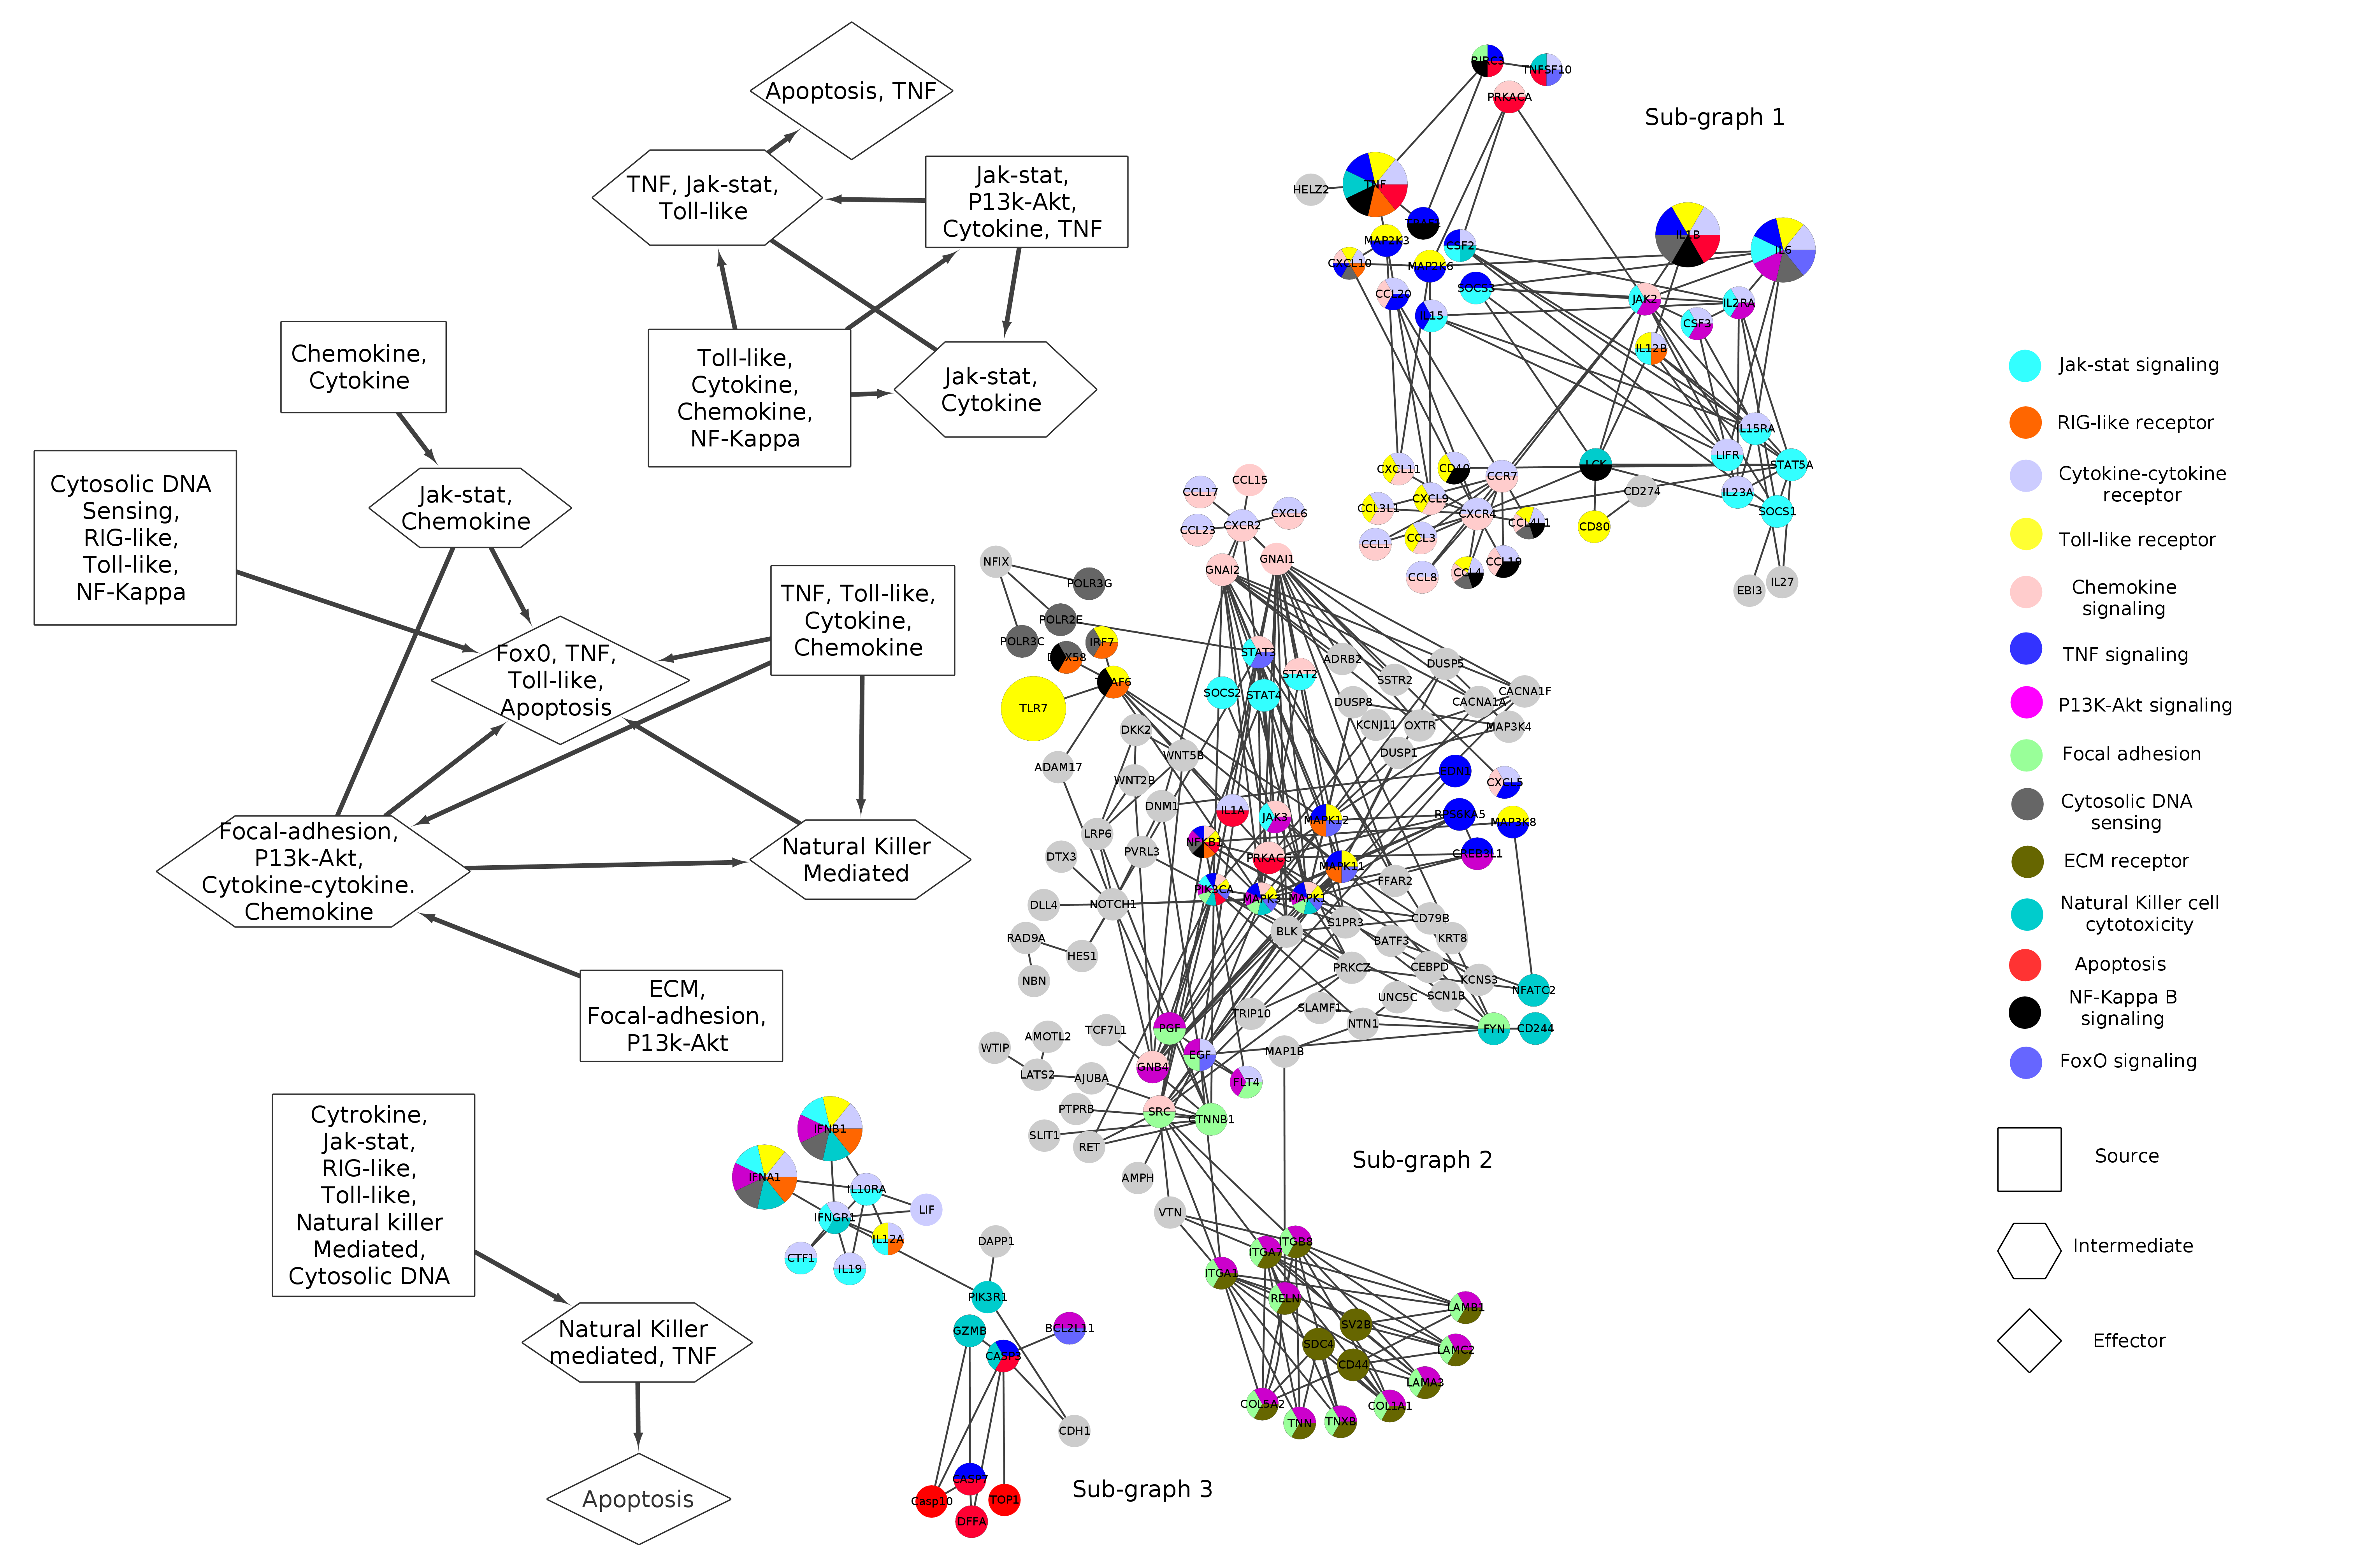
\includegraphics[width=1.05\linewidth]{SeperatedMergedNetwork.png}
			\caption{Visualisation of the three modulated
                          sub-graphs identified by MSF at 6~h after
                          EBOV infection in gene detail and their
                          epitomized representation to depict the flow
                          of perturbation in the directed network. The
                          node coloring is associated to KEGG pathways
                          referring to the colors in the legend. The
                          graph edges are from Reactome. Important
                          genes to EBOV infection as from literature
                          are enlarged in the
                          graph.\label{fig:Sub-graph6hpi}}
		\end{minipage}
	}
\end{figure*}




\begin{figure*}[p]
	\centering
	\fbox{
		\begin{minipage}{12 cm}
			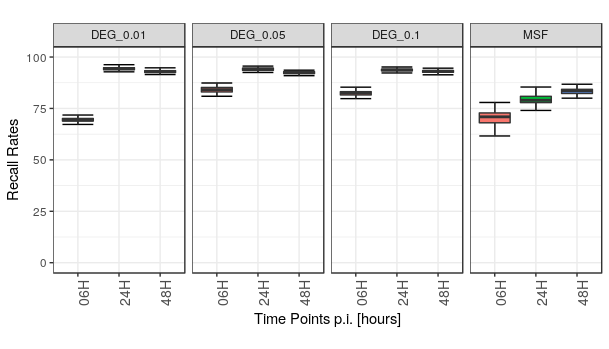
\includegraphics[width=12cm]{DEGvsMSF.png}
			\caption{Shows the percentage of DEG analysis (3 different cut-offs) genes
                          and MSF identified sub-graph genes recall
                          rates for the three different time points of
                          EBOV infection data for 100 simulation where
                          Poisson distributed noise was added to the
                          experimental deduced reads per gene
                          counts.\label{fig:DEGvsMSF}}
			\label{label}
		\end{minipage}
	}
\end{figure*}

\begin{figure*}[p]
	\centering
	\fbox{
		\begin{minipage}{10 cm}
	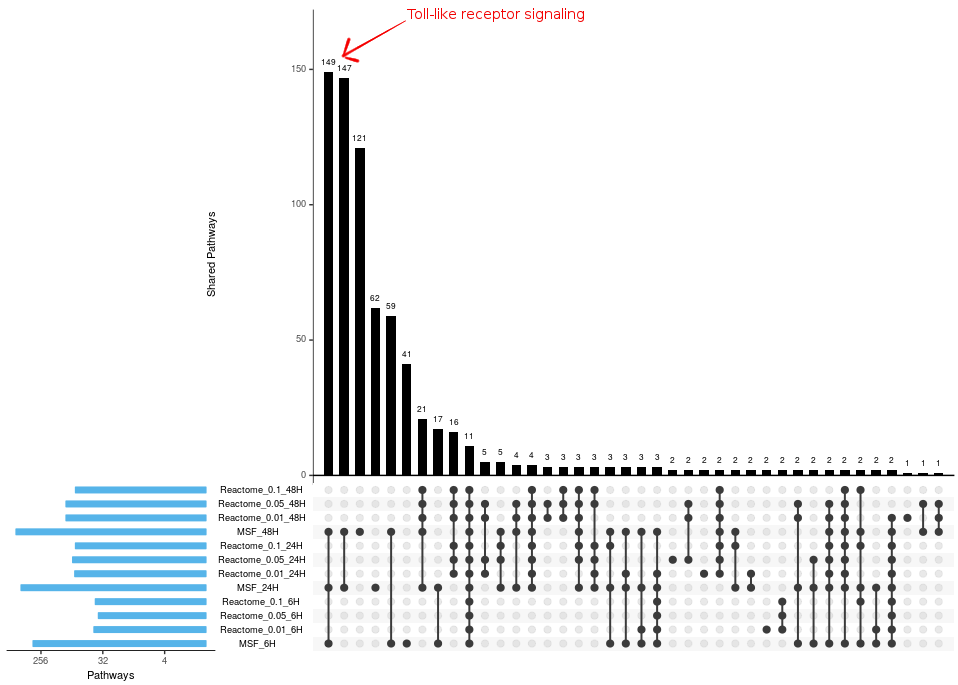
\includegraphics[width=1.0\linewidth]{MSFvsReactomeUpsetPlot}
	\caption{The Upset plot shows the number of common pathways between different time-point and cut offs. }
	\label{fig:msfvsreactome}
\end{minipage}
}
\end{figure*}



\begin{table*}[]
	\centering
	\caption{Comparison of connected sub-graphs of modulated genes
          in the global network between the analysis results of
          \texttt{MSF} and mapping the raw list of differentially
          expressed genes from the standard edgeR analysis, applying
          different p-value cut-offs, onto the network. }
	\label{tab:rawVsHartung}
	\begin{tabular}{lll}
		\hline
		\multicolumn{1}{|l|}{}                            & \multicolumn{1}{c|}{\textbf{Total number of}}       & \multicolumn{1}{c|}{\textbf{Number of connected}}      \\
                \multicolumn{1}{|l|}{}                            & \multicolumn{1}{c|}{\textbf{genes in network}}      & \multicolumn{1}{c|}{\textbf{sub-graph in network}}     \\ \hline
		\multicolumn{1}{|l|}{\textbf{6hpi}}               & \multicolumn{1}{l|}{}                                                & \multicolumn{1}{c|}{}                 \\ \hline
		\multicolumn{1}{|l|}{edgeR + MSF}                 & \multicolumn{1}{c|}{166}                                             & \multicolumn{1}{c|}{3}                \\ \hline
		\multicolumn{1}{|l|}{edgeR (p-value $\leq$ 0.1)}  & \multicolumn{1}{c|}{123}                                             & \multicolumn{1}{c|}{39}               \\ \hline
		\multicolumn{1}{|l|}{edgeR (p-value $\leq$ 0.05)} & \multicolumn{1}{c|}{123}                                             & \multicolumn{1}{c|}{47}               \\ \hline
		\multicolumn{1}{|l|}{edgeR (p-value $\leq$ 0.01)} & \multicolumn{1}{c|}{112}                                             & \multicolumn{1}{c|}{53}               \\ \hline
		\multicolumn{1}{|l|}{\textbf{24hpi}}              & \multicolumn{1}{c|}{}                                                & \multicolumn{1}{c|}{}                 \\ \hline
		\multicolumn{1}{|l|}{edgeR + MSF}                 & \multicolumn{1}{c|}{438}                                             & \multicolumn{1}{c|}{4}                \\ \hline
		\multicolumn{1}{|l|}{edgeR (p-value $\leq$ 0.1)}  & \multicolumn{1}{c|}{325}                                             & \multicolumn{1}{c|}{76}               \\ \hline
		\multicolumn{1}{|l|}{edgeR (p-value $\leq$ 0.05)} & \multicolumn{1}{c|}{305}                                             & \multicolumn{1}{c|}{102}              \\ \hline
		\multicolumn{1}{|l|}{edgeR (p-value $\leq$ 0.01)} & \multicolumn{1}{c|}{262}                                             & \multicolumn{1}{c|}{110}              \\ \hline
		\multicolumn{1}{|l|}{\textbf{48hpi}}              & \multicolumn{1}{c|}{}                                                & \multicolumn{1}{c|}{}                 \\ \hline
		\multicolumn{1}{|l|}{edgeR + MSF}                 & \multicolumn{1}{c|}{320}                                             & \multicolumn{1}{c|}{3}                \\ \hline
		\multicolumn{1}{|l|}{edgeR (p-value $\leq$ 0.1)}  & \multicolumn{1}{c|}{226}                                             & \multicolumn{1}{c|}{39}               \\ \hline
		\multicolumn{1}{|l|}{edgeR (p-value $\leq$ 0.05)} & \multicolumn{1}{c|}{207}                                             & \multicolumn{1}{c|}{62}               \\ \hline
		\multicolumn{1}{|l|}{edgeR (p-value $\leq$ 0.01)} & \multicolumn{1}{c|}{173}                                             & \multicolumn{1}{c|}{67}               \\ \hline
	\end{tabular}
\end{table*}




\end{document}
